% Variante ohne Aufdeck-Effekte \documentclass[handout]{beamer}
% http://groups.google.de/group/comp.text.tex/browse_thread/thread/6ac8485c7a17252a
\documentclass{beamer}
%\documentclass[draft]{beamer}
\usepackage[T1]{fontenc}
\usepackage[utf8]{inputenc}
\usepackage[ngerman]{babel}
\usepackage{listings}
\usepackage{color}

\mode<presentation>{\usetheme{Copenhagen}}

\title{Das Carrierpigeon-Projekt}
\author{Julius Adorf, Marek Kubica, Hong-Khoan Quach}

\date{13.11.2009\\ -  \\ETI-Projekt GP 8 \\ Sommersemester 2009}
\institute{Technische Universität München}

% Entfernen der Navigationsleiste
% Siehe auch http://wiki.ubuntuusers.de/ubuntuusers/LaTeX-Beamer
\beamertemplatenavigationsymbolsempty

% ftp://ftp.tex.ac.uk/tex-archive/macros/latex/.../listings/listings.pdf
\lstset{language=C}
\lstset{numbers=left}
\lstset{
    basicstyle=\small,
    keywordstyle=\color[rgb]{0.2,0.8,0.2}
    }

\begin{document}

\frame{\titlepage}

% --------------------------
\frame{

    \frametitle{Idee}
    
    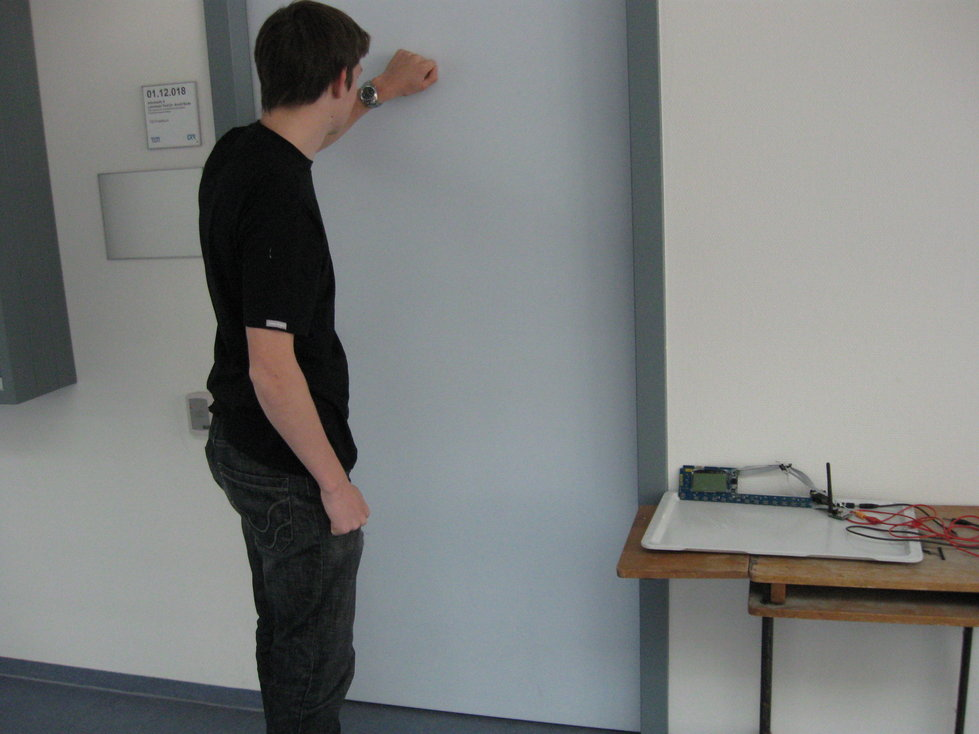
\includegraphics[scale=0.4]{media/story/1.JPG}
    \pause
    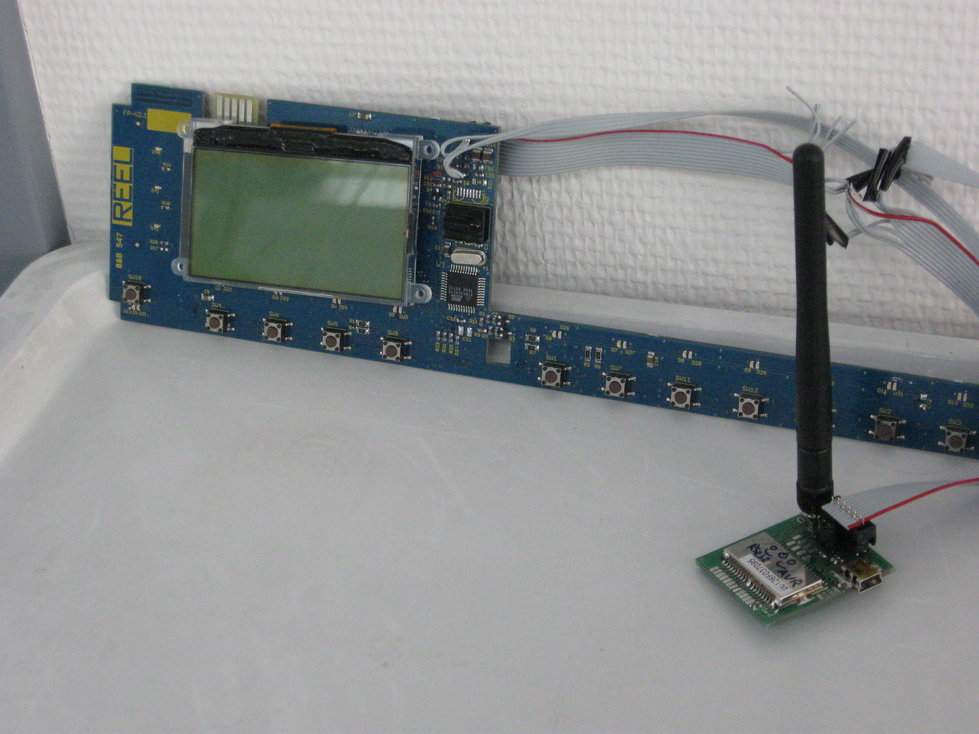
\includegraphics[scale=0.4]{media/story/2.JPG}\
    \pause
    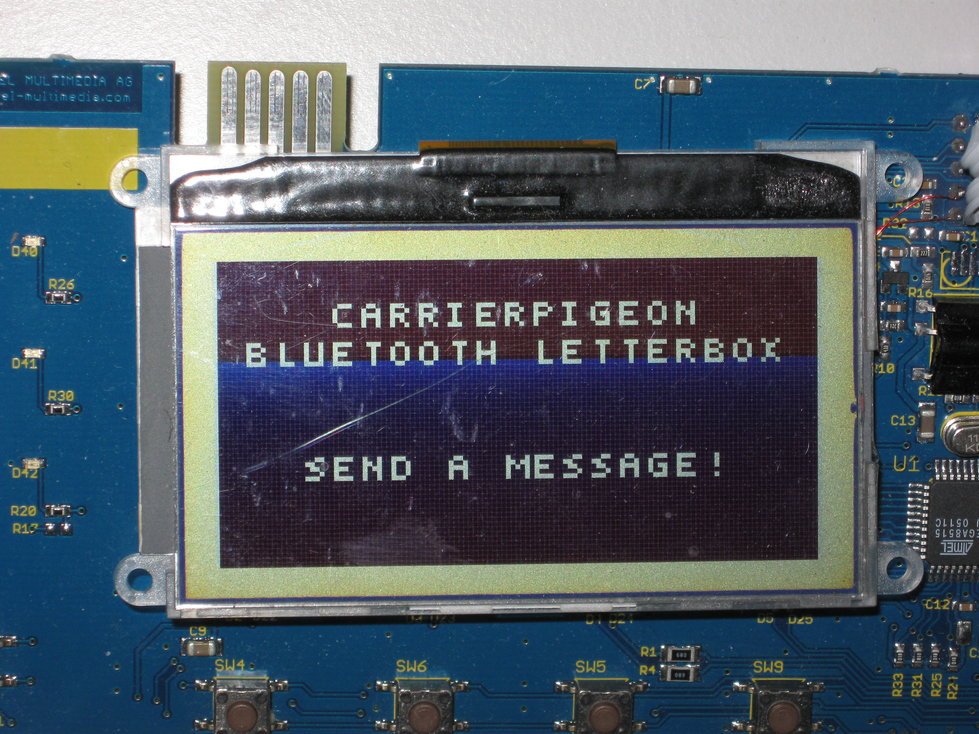
\includegraphics[scale=0.4]{media/story/3.JPG}
    
    
    %[pausesections] <- does not work....

}

\frame{
    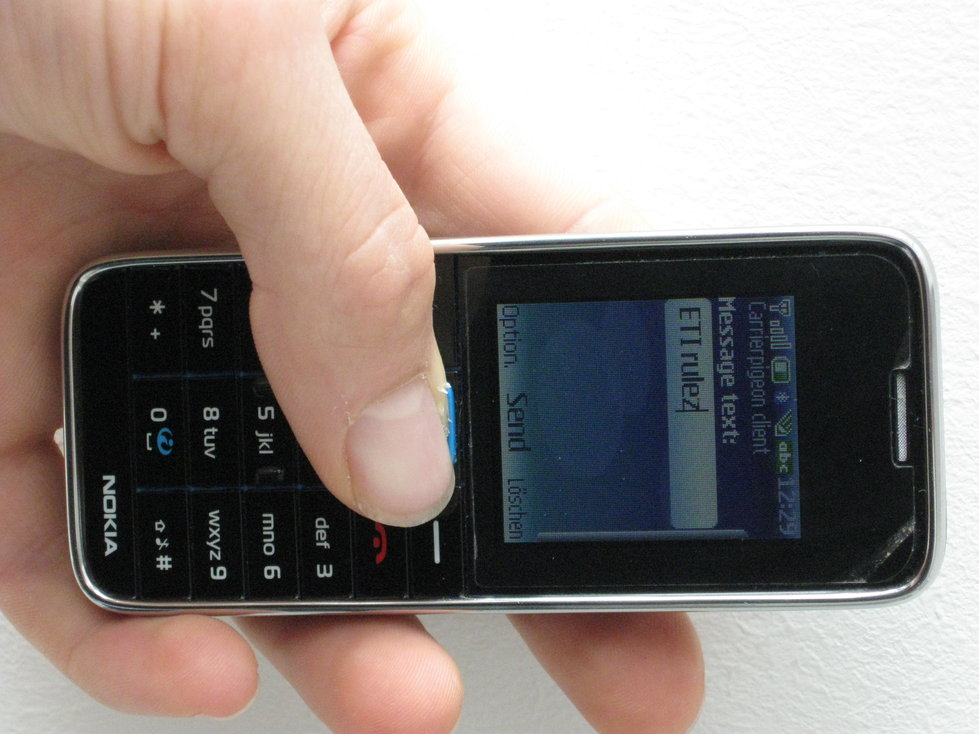
\includegraphics[angle=90, scale=0.5]{media/story/4.JPG}
    \pause
    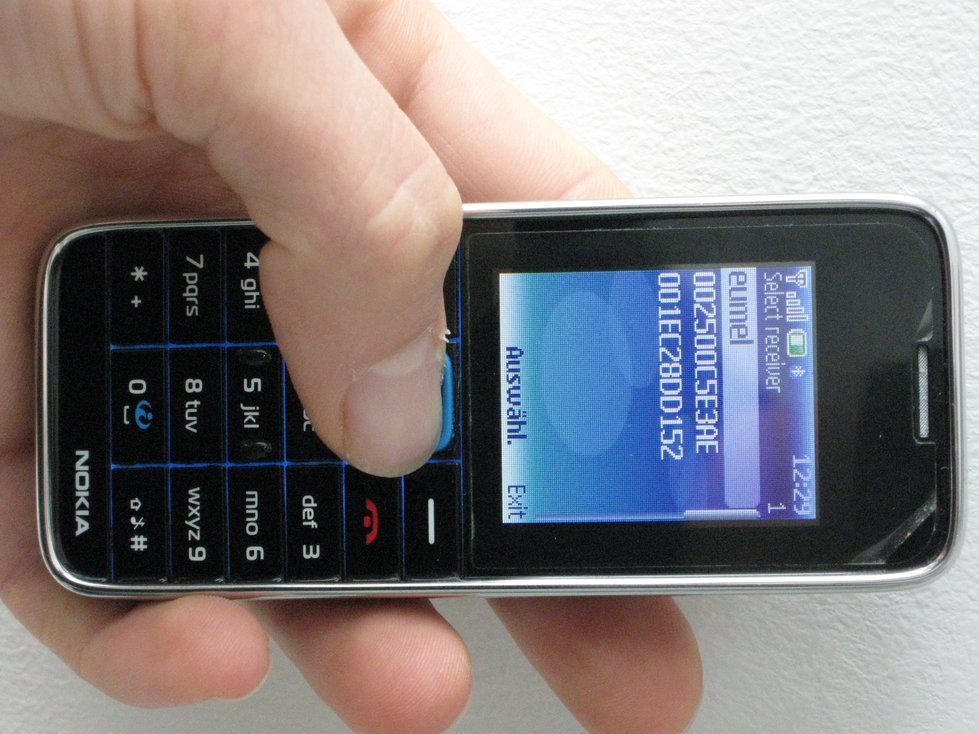
\includegraphics[angle=90, scale=0.5]{media/story/5.JPG}
    
    
}

\frame{
    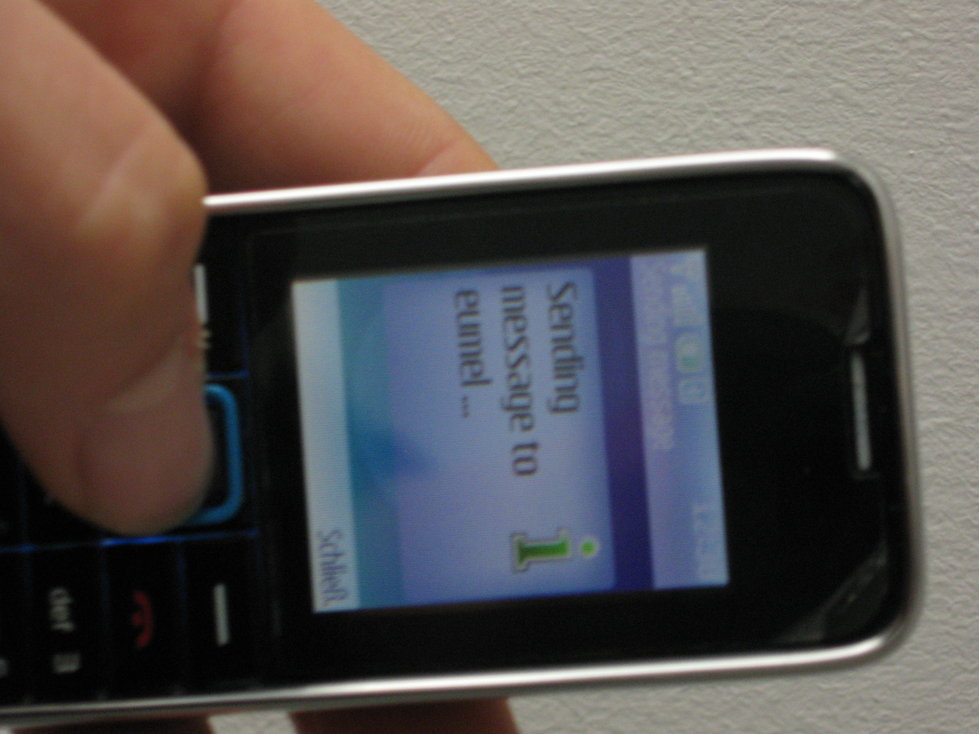
\includegraphics[angle=90, scale=0.5]{media/story/6.JPG}
    \pause
    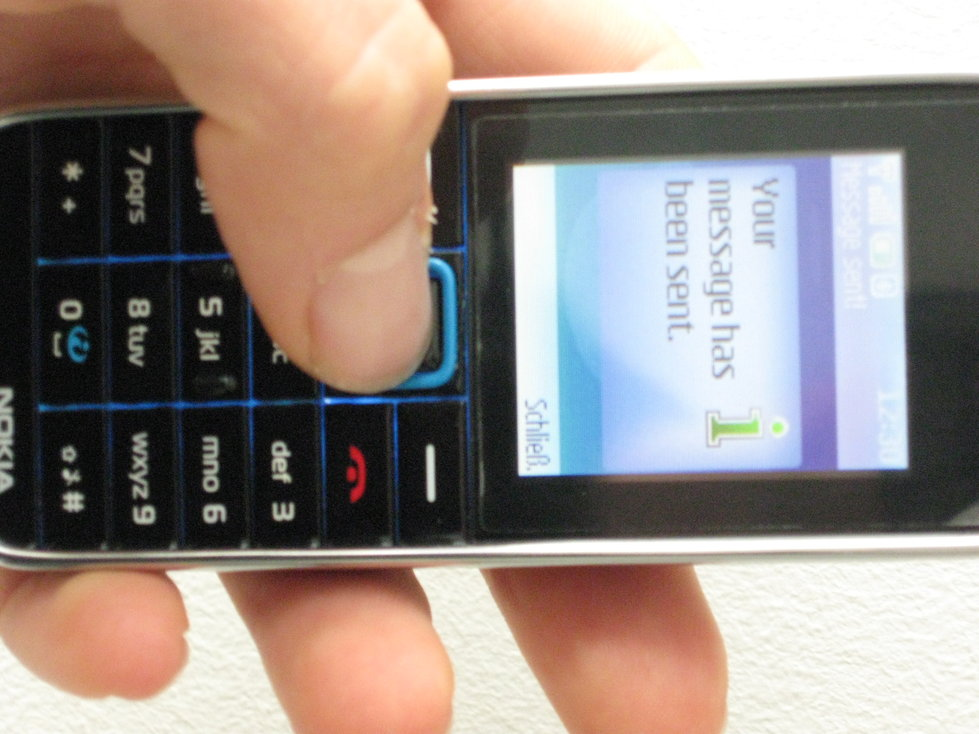
\includegraphics[angle=90, scale=0.5]{media/story/7.JPG}
}

\frame{
    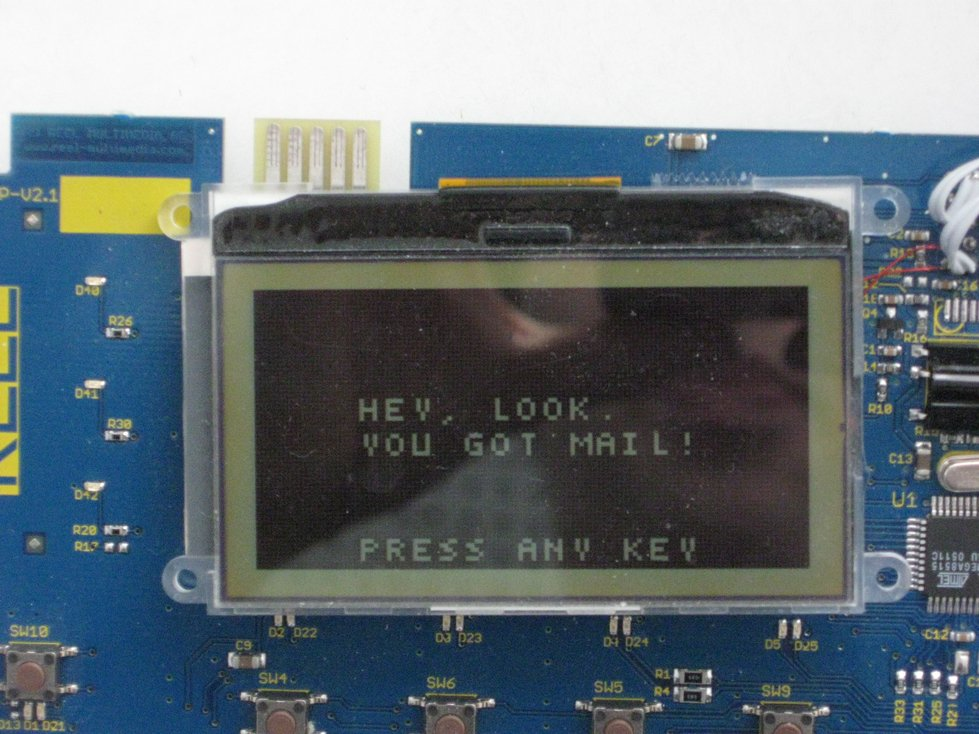
\includegraphics[scale=0.2]{media/story/8.JPG}\
    \pause
    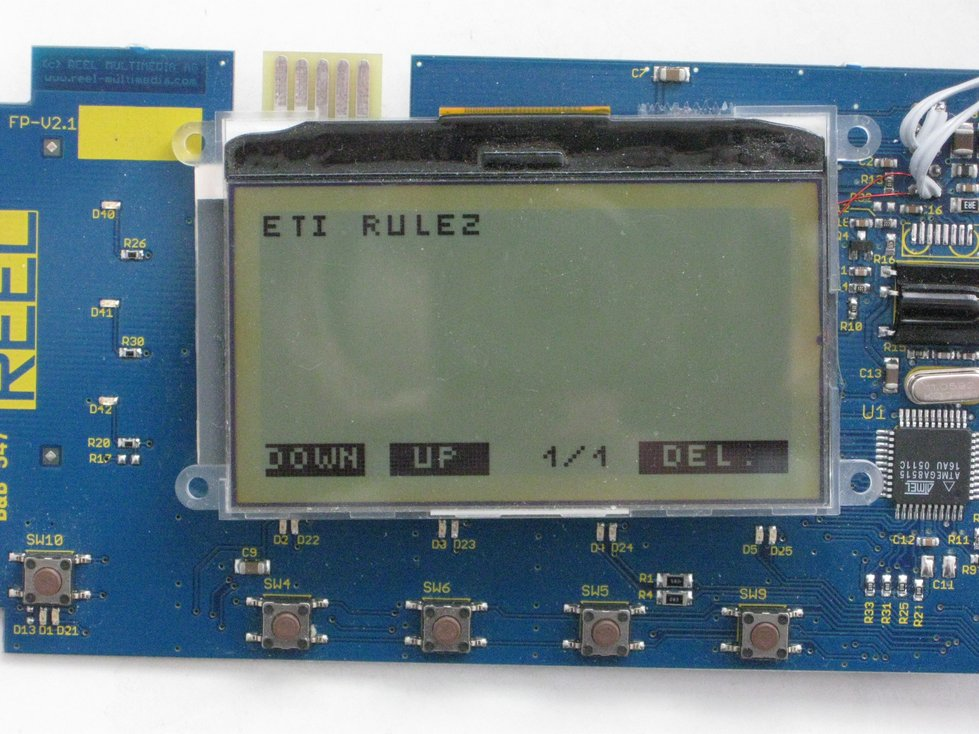
\includegraphics[scale=0.2]{media/story/9.JPG}\
}

\frame{

    \frametitle{Architektur}
    
}

\frame{

    \frametitle{Lösungswege}

}

\frame{

    \frametitle{Ziele - Sicherheit und Stabilität}

    \begin{itemize}
        \item Bluetooth-Clients dürfen keinen Schaden anrichten 
        \item Programm darf nicht abstürzen 
        \item Neustart soll immer möglich sein
    \end{itemize}


    % 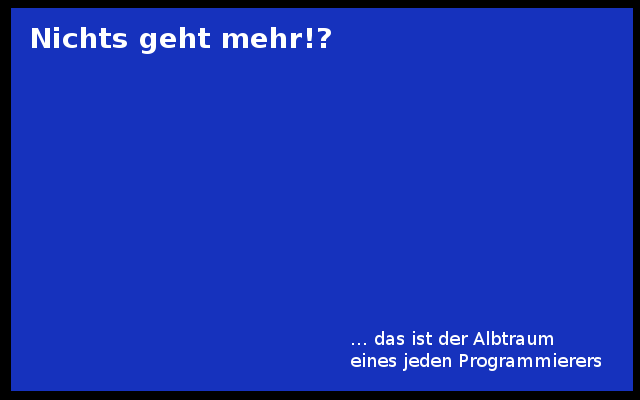
\includegraphics[scale=0.4]{media/bluescr}

}

\frame{
    \frametitle{Mittel - Stabilität}

    \begin{itemize}
        \item der Server hat immer Recht 
        \item Timeouts sorgfältig programmiert
        \item Globale Variablen vermieden
        \item While-Schleifen vermieden
        \item While-Schleifen überprüft
    \end{itemize}

}

\frame{

    \frametitle{Herausforderung: Speicherverwaltung}

    \includegraphics[scale=0.4]{media/eeprom}

}

\frame{
    
    \frametitle{Herausforderung: sicheres Einschalten}

   \begin{itemize}
        \item Nachrichtenzähler überprüfen
        \item Blockzeiger überprüfen
        \item Blockzeiger auf Duplikate überprüfen
    \end{itemize}

    Damit der Techniker nicht zum Hausbesuch kommen muss.

}

\frame{

    \frametitle{Ausbaumöglichkeiten}

\begin{figure}
    \includegraphics[scale=0.2]{media/idea}
\end{figure}

   \begin{itemize}
        \item Protokollerweiterung 
        \item Mehr Speicher einbauen 
        \item Korrekte Zeilenumbrüche
        \item Automatische Tests mit GNU Debugger und AVR-Simulator 
    \end{itemize}

}

\frame{

    \frametitle{Fazit}

    \begin{figure}
        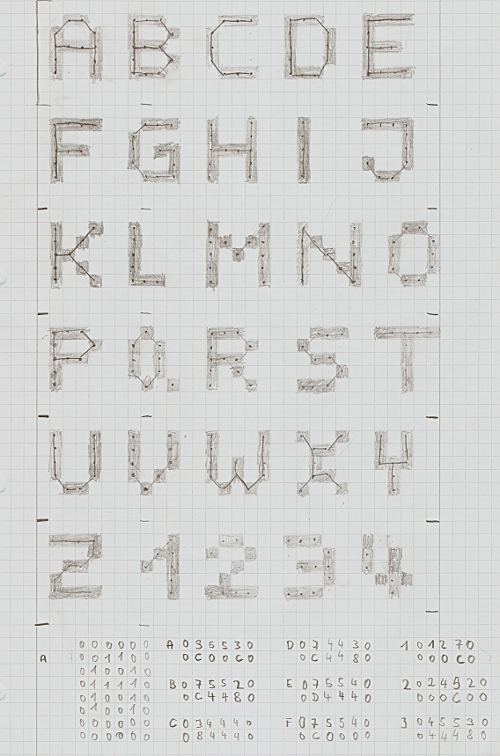
\includegraphics[scale=0.6]{media/font}
    \end{figure}

   \begin{itemize}
        \item Anforderungen erfüllt!
        \item Einsatz verschiedener Techniken ...
        \item ... was am Ende auch funktioniert hat!
    \end{itemize}

}

\frame{

    \frametitle{Ausprobieren}

    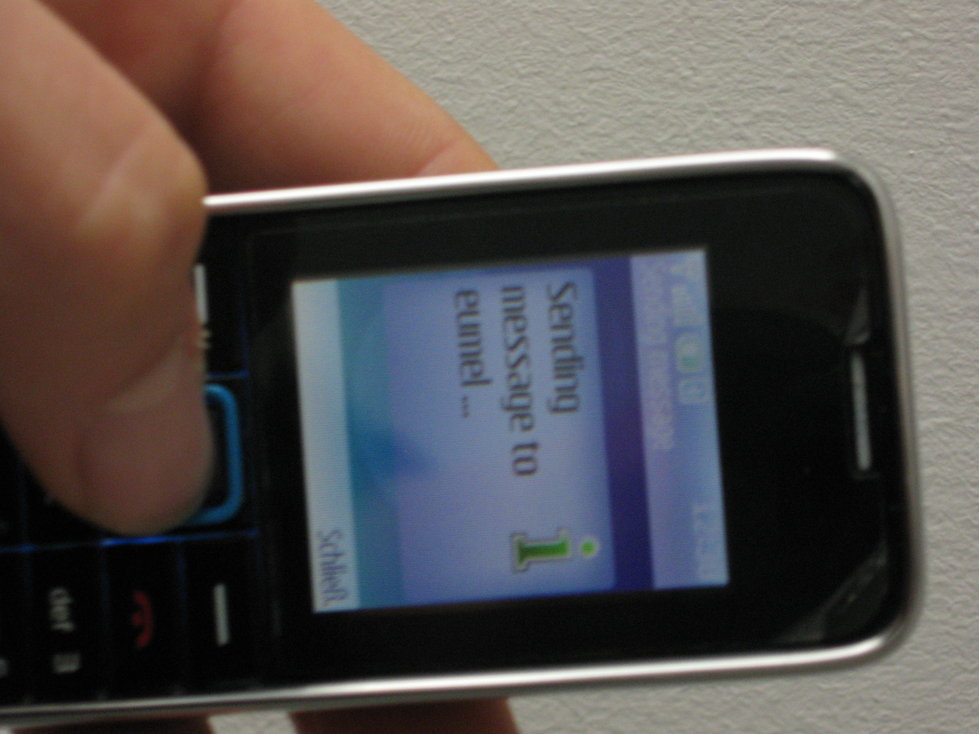
\includegraphics[angle=90, scale=0.24]{media/story/6.JPG}

    Wer es ausprobieren mag:

   \begin{itemize}
        \item http://bitbucket.org/jeadorf/carrierpigeon/downloads
        \item Mobile-Client (JAR und evtl. JAD) herunterladen und auf das Handy spielen
    \end{itemize}

}

\frame{

    % empty
    \begin{center}
    ( . )
    \end{center}
}


%
% --------------------------

\frame{

    \frametitle{Toolchain}


    \begin{tabular}{|r||l|}
        \hline
        Hardware & ATmega 8515, BTM-222, ST7565 LCD, AVRISP2 \\
        \hline
        Languages & C, Java, Python\\
        \hline
        Framework & Java Micro Edition, Peter Fleury's UART library\\
        \hline
        Compilation & {\tt avr-gcc, avr-objcopy, avr-strip, avrdude,} \\
                    & {\tt avr-nm, avr-size, splint, python, ant} \\
        \hline
        Helpers & {\tt
       hcitool, rfcomm, gtkterm, jpnevulator
    } \\
        \hline
    \end{tabular}

    
}

\end{document}

